\title{Lab report on subject 001}
\author{
        John~O.~Woods,~Ph.D. \\
            \and
        Amie~E.~Hinds,~M.S. \\
            \and
        Luke Shafer,~M.S. \\
        R.~Daneel~Olivaw~Corporation\\
        908 Winston St., Suite \textsc{g} \\
        Houston, Texas 77009
}
\date{\today}

\documentclass[10pt]{article}

\usepackage{graphicx}
\usepackage{amsthm}
\usepackage{enumerate}

\theoremstyle{definition}
\newtheorem{term}{Term}

\begin{document}
\maketitle

%\begin{abstract}
%This is the paper's abstract \ldots
%\end{abstract}

\section{Objective}
Our contracted objective was to ascertain uses, if any, of our subjects.
Instruction prioritized minimizing damage to the subjects, and using the least destructive analyses possible.

\section{Introduction}
The subjects were recovered from certain near-earth asteroids, and appear to be artifacts of some sort.
They appear to be of similar technological origin, having common components and visually similar design.
The intended use of these objects is unknown.
The subjects arrived with an arbitrary numbering scheme, which we have adopted.

Subjects 001--004 and 007--008 all contain minerals mounted in the center of a metallic setting, whereas subjects 005 and 006 appear to be hardware mounts for a glass-like material.
The minerals and the glass appear to have been polished to a high gloss.

We propose a simple taxonomy which simplifies the descriptive aspect of our task; it groups the subjects into two types based on the central component (mineral or glass).
However, we acknowledge that this taxonomy may highlight an arbitrary aspect of the subjects, and multiple independent taxonomies could be developed which emphasize other traits.
We therefore utilize this taxonomy --- shown in Fig.~\ref{fig:taxonomy} and discussed in the following section --- solely for convenience.

\begin{figure}
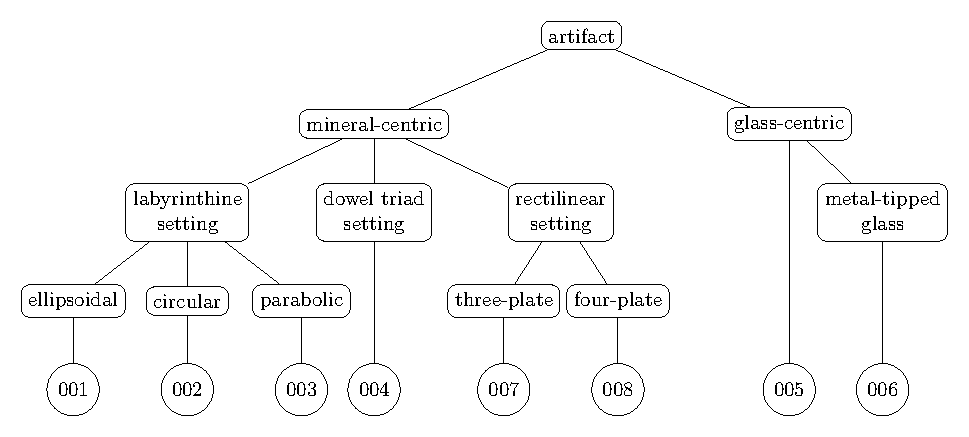
\includegraphics[width=1.0\textwidth]{taxonomy.pdf}
\caption{\label{fig:taxonomy}\textbf{We classified the artifacts into a taxonomy whose first level centers on what we perceive to be the central component, which is either a refined mineral or some type of artificial glass.} For the mineral-centric subjects, the second level describes the setting for the gem, which is itself mounted in place on some sort of device. One of the glass-centric subjects has metal `tips' on the glass piece, and it receives its own category. We have not included the mounts in this taxonomy, as they each --- with the exception of those for 005 and 006 --- appear wholly unique. Indeed, the mounts for 005--006 are much less distinguishable from what we refer to as the settings. The terminology is defined in Section~\ref{sec:taxonomy}. The last row in the taxonomy provides the subject number, such that each subject has its own unique classification. For example, subject 001 is the sole artifact can be uniquely described, at least among those artifacts of which we are aware, as \texttt{artifact/mineral/labyrinthine/ellipsoidal}. }
\end{figure}

%Subjects 001--004 and 007--008 consist of two parts, which we refer to as the mineral and the setting. Subjects 005--006 likewise have two components; however, in lieu of a mineral, the setting serves as a mount for what appears to be glass.

\subsection{Taxonomy}\label{sec:taxonomy}
Our taxonomy is best understood using the following terminology.

\begin{term}
\emph{Gem} is the term we use to describe the objects of apparently mineral origin.
\end{term}

As the minerals in subjects 001--004 and 007--008 are gem-like, we have adopted some identifying methods and terns from gemology, which we do not define here.

\begin{term}
The \emph{setting} is the piece whose metal contacts are in immediate contact with the gem or glass. It may be either wholly metallic or partially. There is a layer of what may be either oxidation or some sort of protective coating (which we will refer to simply as oxidation hereafter) on several of the settings; this layer appears to have been scraped off on the settings' edges and corners.
\end{term}
\begin{term}
\emph{Labyrinthine} describes the patterns in the metal of some of the settings, which resemble either mazes or perhaps circuit boards. These have the most visible oxidation.
\end{term}
\begin{term}
\emph{Dowel triad} partially describes the setting for subject 004, which are three identical metal rods which pin the gem in the center of a short hollow cylinder.
\end{term}
\begin{term}
\emph{Rectilinear} describes the mounts for 007 and 008, which have linear edges and primarily right (and some $45^\circ$) angles.
\end{term}
\begin{term}
The \emph{mount} is the piece to which the setting is attached, except in two cases: the glass-centric subjects, in which the mount and setting are not distinct; and the rectilinear subjects, which have no mount.
\end{term}
\begin{term}
The \emph{connectors} are uniform metallic pins which resemble an electronic interface, such as one might find on a computer processor or microcontroller. These are of differing sizes and are present on all subjects except for 007 and 008.
\end{term}
\begin{term}
The \emph{plates} are identical, parallel metal quadrilaterals which enclose the gems in subjects 007 and 008. On one end of each is a single plate; on the other end there are either two (007) or three (008). We thus refer to these respectively as three-plate and four-plate.
\end{term}

\section{Methods}
We endeavored to obtain as much information about the subjects as possible with as little potential impact on it as was feasible.

The mineral's properties may be categorized as either physical or optical.
We used a $10\times$ hand lens and ultraviolet light to discern basic physical properties.
For optical properties, a $45\times$ polarizing gemological microscope, a dichroscope, and a refractometer were employed.


\section{Results}
Rather than refer to the objects only by their numbers, we identify them using identifying terms from their taxonomies.

\subsection{Central objects}
\subsubsection{Basic physical characteristics of the central objects}

\begin{enumerate}[(001)]
\item \textbf{Ellipsoidal labyrinthine:} The gem is yellow in color, transparent, and has a vitreous luster.
    Unfortunately, certain diagnostic features such as cleavage and fracture were obliterated with the cutting and polishing by --- we presume --- the creators of this artifact.
    Other physical properties such as hardness and specific gravity could not be tested due to our instructions not to abrade the subject.
\item \textbf{Circular labyrinthine:}
\item \textbf{Parabolic labyrinthine:}
\item \textbf{Dowel triad:}
\item \textbf{Glass-centric:}
\item \textbf{Metal-tipped glass-centric:}
\item \textbf{Three-plate rectilinear:}
\item \textbf{Four-plate rectilinear:}
\end{enumerate}

\subsubsection{Optical characteristics of the central objects}
\begin{enumerate}[(001)]
\item \textbf{Ellipsoidal labyrinthine:} Using the tools outlined above, we determined that the optical properties of the mineral are similar to those of quartz.
    Specifically, we measured the refractive index (\textsc{ri}) to be exactly 1.55.
    We used a polarizing microscope and determined that the mineral is anisotropic; the dichroscope allowed us to determine that the mineral is doubly refractive.
\item \textbf{Circular labyrinthine:}
\item \textbf{Parabolic labyrinthine:}
\item \textbf{Dowel triad:}
\item \textbf{Glass-centric:}
\item \textbf{Metal-tipped glass-centric:}
\item \textbf{Three-plate rectilinear:}
\item \textbf{Four-plate rectilinear:}
\end{enumerate}

\subsubsection{Electromagnetic properties}
We attempted to take measurements using a cheap digital multimeter with sensor wires applied to various contacts on subject 004.
First, we verified that the contacts were conductors, by applying the wires at the same time to the same contact; we measured a resistance of 0 $\Omega$.
We next attempted to apply the multimeter wires to adjacent contacts, but were unable to find any that would pass a measurable current.
As each subject possessed hundreds contacts, we were unable to systematically investigate all of the tens of thousands of combinations of contacts on any one artifact --- let alone all of them. 

It is possible that the subjects' electrical internals have been destroyed, but it seems strange that devices capable of non-electromagnetically-induced anti-gravitation should have electrical internals that could so easily have been damaged.
It is also possible that the contacts are connected in triples rather than pairs --- such as with transistors or vacuum tubes --- or that they function only in some specific combination.
It is not clear why devices which appear not to rely on electromagnetism even need electrical contacts; perhaps they are something else entirely.

The black portions of the subjects do not appear to conduct; neither do the polished stones, nor the apparent metallic ends on subject 006.

Obviously, whether an object possesses conductance or not is relative rather than absolute, but we were reluctant to apply higher voltages to the subjects.

We observed that subjects 007 and 008 (the rectilinear artifacts) produce a stronger than expected magnetic field based upon their apparent composition, and confusingly, the subjects' dipole moments appear to rotate.
Not only do the dipole moments rotate, but they does so seemingly \textit{in tandem} with the placement of either a magnetometer or a simple compass relative to whichever artifact is being examined.

\subsection{Fundamental force irregularities}
While measurement of an object's mass seems so trivial as to belong in a grade-school lab report, our observations of the subjects have led us to exercise a great deal of skepticism regarding the standard methods.
For example, a digital laboratory scale expresses its measurement in grams, which is a mass measurement --- but, in fact, the scale provides a measurement of force, not mass, and converts according to a calibration to the local gravitational field.

Several assumptions are implicit in such a measurement:
\begin{enumerate}
\item The object is subject only to gravitational force, and other forces (\textit{e.g.} magnetic) are tiny in comparison.
\item The object contains no regions that are of lower density than the atmosphere. Imagine, for example, a chamber containing helium at atmospheric pressure. Such a chamber would have an apparent weight less than that of an equivalent chamber containing standard atmosphere. Similarly, a chamber containing nothing --- a vacuum --- would weigh less than either the helium chamber or the atmosphere-containing chamber.
\item The object's temperature is at equilibrium with the environment (though this is only significant for gases and not solid objects, we mention it to be exhaustive in the face of confusing experimental results).
\end{enumerate}

Based on our observations, none of these assumptions necessarily apply to the objects in question.
Firstly, we note the stronger than expected magnetic field and rotating dipole moment on some subjects.

We next attempted to individually observe the weight of a number of subjects, but found that the measured value changed as we re-oriented them.
(Again, we lacked sufficient time to perform the same tests on all subjects, so the following remarks refer only to the circular labyrinthine subject, 002.)
When we cycled back through the orientations a second time, the apparent weight differed by up to around five percent from the first set of measurements.
When tested in the early afternoon, the scale recorded an average mass of 40.2 grams with a standard deviation of 1.2 grams.
We repeated the experiment an hour later and recorded an average mass of 41.5 grams --- again with a standard deviation of 1.2 grams.
Time constraints rather limited our ability to discern any meaningful trend.

However, one of us (Amie) noticed a peculiarity: subject 005 behaves extremely oddly when placed in a centrifuge.
Its mean measured mass was 24.1 grams, but we observed that a 25-gram weight placed on the opposite end of a 0.25-meter centrifuge from the artifact produced a substantial imbalance.

These results are fairly confusing, and explaining why requires us to go back to first principles.
Newton's first and second laws are, respectively:
%
\begin{eqnarray}
\mathbf{F} &=& m \mathbf{a} \\
 &=& \dot{\mathbf{p}}\,\textrm{,}
\end{eqnarray}
%
where
%
\begin{equation}
\mathbf{p} = m \mathbf{v}
\end{equation}
%
is the momentum.
%
The two laws can be related to each other by taking the time derivative of the momentum,
%
\begin{equation}
\dot{\mathbf{p}} = m \dot{\mathbf{v}} = m \mathbf{a} = \mathbf{F}\,\textrm{,}
\end{equation}
%
and so the change in momentum over time turns out to be the force.
Thus, centripetal force arises from a change in the momentum $\mathbf{p}$ of an object of mass $m$.
However, subject 005's centripetal force seems not to be predictable from its mass --- that, or its mass is not predictable from its weight, which is a mind-bogglingly disorienting concept.

We found that subject 006 behaved similarly to 005, but none of the other subjects seemed to produce such an observable imbalance.
We hesitate to even report these results because they seem so inconsistent with our understanding of the laws of physics.

Had we a much greater allowance of time, our next step would be one of the following:
\begin{enumerate}
\item Measure the weights and accelerations (when dropped) of the subjects at different latitudes, along with the gravity at those same locations. For example, at our geodetic latitude $\phi=29.801445^\circ$, gravitational acceleration should be around 9.792 $\textrm{m}/\textrm{s}^2$ (using a simple gravity model rather than a measurement), and centripetal acceleration should amount to 0.029 $\textrm{m}/\textrm{s}^2$ (about a quarter of a percentage reduction in gravity). Near the poles, the centripetal acceleration will be closer to zero, and at the equator, 0.034 $\textrm{m}/\textrm{s}^2$.
\item Measure the mass using the subjects' momentums when attached to a spring --- or hydraulic shock absorber --- of known spring constant $k$. This strategy has been employed, for example, to weigh astronauts in microgravity, such as aboard the International Space Station. Such a measurement would likely require an extremely sensitive hydraulic device given the size of the objects in question.
\end{enumerate}

Let us take as given that some or all of these devices possess an advanced faculty allowing them either to negate inertia or to reduce the influence of gravity upon themselves (or both).
We can think of a few possible uses of such properties, among them:
\begin{itemize}
\item \textbf{Propulsion.} We can imagine several concepts for propulsion using such faculties, among them the old science fiction concept of anti-gravity. Even with a device which functions by inertia negation, it would be possible to possible to move through space through mechanical means rather than using a rocket.
\item \textbf{Energy production,} though of course depending entirely upon details of the functioning of these faculties of which we have no insight. Indeed, most of these possibilities depend a great deal on the power source for these devices.
\item \textbf{Navigation.} An accelerometer in free fall experiences no gravity and thus measures zero acceleration (even though it is clearly accelerating). An accelerometer which could reduce its interaction with a gravitational field could then precisely measure that field as it moves through space.
\item \textbf{Weaponry.} We hesitate to mention it, but a device which can reduce its momentum may also be able to increase its momentum --- and we can't rule out the possibility of increasing the amount of gravitational force experienced, either.
\end{itemize}

\subsection{Radioactivity}
Our observations consistently showed the subject to be unremarkable in terms of its alpha, beta, and gamma emissions.

\section{Conclusions}\label{conclusions}
The subject responds unexpectedly to stimuli, based on its behavior in water and in the presence of a magnetometer.

%The physical and optical properties of the mineral are consistent with those of lime citrine variety quartz.
%Therefore, we believe it reasonable to consider other properties typically associated with quartz, which is known to have piezoelectric and pyroelectric properties.
%These properties could help explain some of the unusual behaviors, such as the transmission of heat while submerged.
%Given additional time, we recommend targeting investigations toward these properties.
 
The four hours of study we were permitted on the subject were insufficient for fully interrogating the range of possibilities produced by our testing, and the tests we performed have produced more questions than answers.

We urge extreme caution when transporting the subjects due to their likely unpredictable behavior in a gravitational field.
It is unclear how the artifacts would behave, for example, in orbit or on the way to orbit.\footnote{This type of information was not recorded when the subjects were initially retrieved from the various near-earth asteroids where they were found. Frustratingly, the operators of the inbound re\"entry vehicle would not provide us with navigation filter logs, arguing that the proprietary nature of their flight software and propulsion systems `regrettably' did not allow them to share those data.}

%\bibliographystyle{abbrv}
%\bibliography{main}

\end{document}